%%%%%%%%%%%%%%%%%%%%%%%%%%%%%%%%%%%%%%%%%
% Jacobs Landscape Poster
% LaTeX Template
% Version 1.1 (14/06/14)
%
% Created by:
% Computational Physics and Biophysics Group, Jacobs University
% https://teamwork.jacobs-university.de:8443/confluence/display/CoPandBiG/LaTeX+Poster
%
% Further modified by:
% Nathaniel Johnston (nathaniel@njohnston.ca)
%
% This template has been downloaded from:
% http://www.LaTeXTemplates.com
%
% License:
% CC BY-NC-SA 3.0 (http://creativecommons.org/licenses/by-nc-sa/3.0/)
%
%%%%%%%%%%%%%%%%%%%%%%%%%%%%%%%%%%%%%%%%%

%----------------------------------------------------------------------------------------
%	PACKAGES AND OTHER DOCUMENT CONFIGURATIONS
%----------------------------------------------------------------------------------------

\documentclass[final]{beamer}

\usepackage[orientation=portrait,size=a0,scale=1,debug]{beamerposter} % Use the beamerposter package for laying out the poster
%\usepackage[brazil]{babel}
\usepackage[T1]{fontenc}
\usepackage[utf8]{inputenc}
\usepackage{multirow}
\graphicspath{{figures/}{./}}

\usetheme{confposter} % Use the confposter theme supplied with this template

\setbeamercolor{block title}{fg=ngreen,bg=white} % Colors of the block titles
\setbeamercolor{block body}{fg=black,bg=white} % Colors of the body of blocks
\setbeamercolor{block alerted title}{fg=white,bg=dblue!70} % Colors of the highlighted block titles
\setbeamercolor{block alerted body}{fg=black,bg=dblue!10} % Colors of the body of highlighted blocks
% Many more colors are available for use in beamerthemeconfposter.sty

%-----------------------------------------------------------
% Define the column widths and overall poster size
% To set effective sepwid, onecolwid and twocolwid values, first choose how many columns you want and how much separation you want between columns
% In this template, the separation width chosen is 0.024 of the paper width and a 4-column layout
% onecolwid should therefore be (1-(# of columns+1)*sepwid)/# of columns e.g. (1-(4+1)*0.024)/4 = 0.22
% Set twocolwid to be (2*onecolwid)+sepwid = 0.464
% Set threecolwid to be (3*onecolwid)+2*sepwid = 0.708

\newlength{\sepwid}
\newlength{\onecolwid}
\newlength{\twocolwid}
\newlength{\threecolwid}
\setlength{\sepwid}{0.005\paperwidth} % Separation width (white space) between columns
\setlength{\onecolwid}{0.20\paperwidth} % Width of one column
\setlength{\twocolwid}{0.464\paperwidth} % Width of two columns
\setlength{\threecolwid}{0.708\paperwidth} % Width of three columns
\setlength{\topmargin}{-0.6in} % Reduce the top margin size
%-----------------------------------------------------------

\usepackage{graphicx}  % Required for including images
\usepackage{subcaption}
\usepackage{booktabs} % Top and bottom rules for tables

%----------------------------------------------------------------------------------------
%	TITLE SECTION
%----------------------------------------------------------------------------------------

\title{Selecting scenarios in temporal ensembles}

\author{Guilherme G. Schardong$^1$, Simone D. J. Barbosa$^1$, Waldemar Celes$^1$, \\
Regis Kruel$^2$, Alexandre Emerick$^2$, Luciano Reis$^2$, Ricardo Chaves$^2$ and H\'{e}lio Lopes$^1$}

\institute{$^1$Departamento de Inform\'{a}tica - PUC-Rio\\
$^2$PETROBRAS}

%----------------------------------------------------------------------------------------

\begin{document}

\addtobeamertemplate{block end}{}{\vspace*{1ex}} % White space under blocks
\addtobeamertemplate{block alerted end}{}{\vspace*{1ex}} % White space under highlighted (alert) blocks

\setlength{\belowcaptionskip}{1ex} % White space under figures
\setlength\belowdisplayshortskip{1ex} % White space under equations

\begin{frame}[t] % The whole poster is enclosed in one beamer frame

\begin{columns}[t] % The whole poster consists of three major columns, the second of which is split into two columns twice - the [t] option aligns each column's content to the top

%\begin{column}{\sepwid}\end{column} % Empty spacer column

\begin{column}{\twocolwid}\vspace{-.3in} % The first column

%----------------------------------------------------------------------------------------
%	OBJECTIVES
%----------------------------------------------------------------------------------------

\begin{alertblock}{Objectives}
The goal of this work is to propose a novel approach for the selection of representative elements in a time series ensemble. To this end, we have developed a visualization technique, the Rank Chart, to graph the adherence of each time series of the ensemble to a reference series, such as the P$_{10}$, P$_{50}$ and P$_{90}$ curves.
\end{alertblock}

%----------------------------------------------------------------------------------------
%	INTRODUCTION
%----------------------------------------------------------------------------------------

\begin{block}{Introduction}

Recent developments in simulation techniques have helped researchers better understand and predict several naturally occurring phenomena. To extract any meaningful information from this amount of data, researchers have been developing an array of approaches in several areas of knowledge. Several of these approaches have been applied in the oil industry.

One of the key tasks in reservoir management is the definition of a production strategy \cite{schiozer:2004}. When a strategy is defined, it must be throughly tested to evaluate its performance. A common way to do so is by simulating the strategy coupled with the reservoir models. Several hundred realizations may result from this process due to uncertainties inherent to the models.

Steagall and Schiozer \cite{steagall:2001} propose the use of three classes of models to evaluate the performance of a production strategy: a pessimistic, probable and optimistic models. However the process of selecting this subset of models is a challenging task due to the sheer number of possible outcomes of a simulation. We propose an approach that takes into account a range of time from each simulation and rank its outcomes according to a score function detailed below. We also propose a novel visualization tool to help analyze the adherence of each series to a set of percentile curves (P$_{10}$, P$_{50}$ and P$_{90}$) calculated from the simulations.

\end{block}

%----------------------------------------------------------------------------------------

%----------------------------------------------------------------------------------------
%	TECHNICAL DETAILS
%----------------------------------------------------------------------------------------

\begin{block}{Rank Chart}
The rank chart is a graphical tool to visualize the adherence of a set of time series to a reference curve. The chart is built by iterating through the time steps of the ensemble entities and calculating the distance between each series and the reference up to that step. This distance is then ordered in ascending order and ranked accordingly. This process creates a new set of time series, now composed of the absolute ranks attained by each ensemble entity at each time step. These ranks are then plotted in a two-dimensional plane where the $x$ axis is the time step and the $y$ axis is the rank.
\end{block}

\begin{block}{Selection Approaches}
\begin{itemize}
  \item \textbf{Score selection}: Given the absolute ranking calculated based on the euclidean distance between the entities, we assign a score for each possible rank. For an ensemble of $N$ entities, we use a linear function $f(r) = N - r - 1$, where $\left(r \in \mathbb{N} | r \in [1, N] \right)$ as the score for each rank $r$. We also assign a weight for each simulation time step based on the desired adherence between the candidate models and the references. The definition of this function depends on the type of analysis and behavior of the ensemble itself.
  \item \textbf{Manual Selection}: We can also manually select a set of series by using an auxiliary view, the scenario/distance chart, in order to select the series closest to the chosen percentiles. The selected series are then highlighted in the corresponding fan and rank charts in order to evaluate their behavior.
  \item \textbf{MDS kNN Selection}: By calculating the Multidimensional Scaling (MDS) of the ensemble, we obtain a representantion where the distance of each point is an approximation of the original distances between each series. We can then use this to select the $k$ series whose projections are closest to the projected percentiles.
\end{itemize}
\end{block}

\begin{block}{Experimental Results}
\begin{figure}[H]
  \centering
  \begin{subfigure}[b]{0.8\columnwidth}
    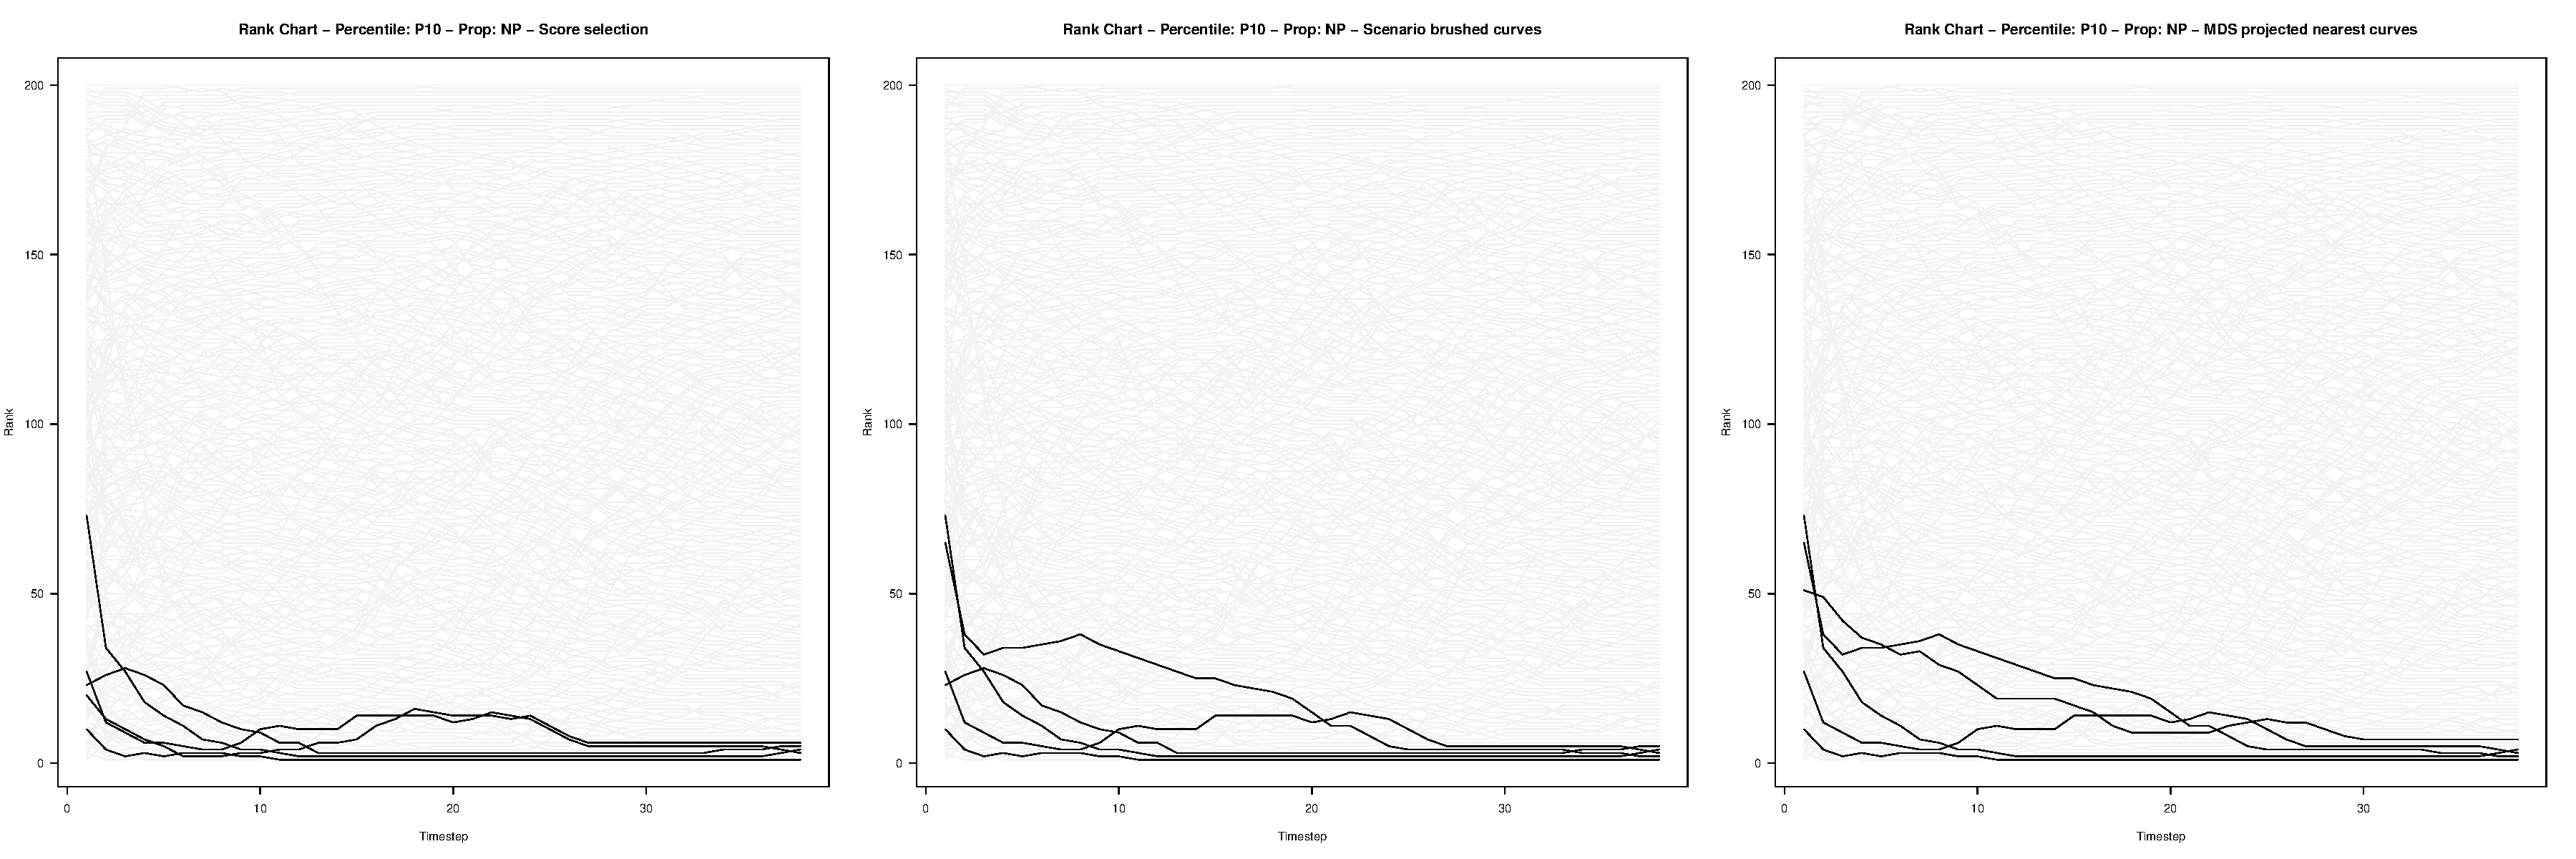
\includegraphics[width=\columnwidth]{rank-score-brush-mds-p10.pdf}
  \end{subfigure}
  \begin{subfigure}[b]{0.8\columnwidth}
    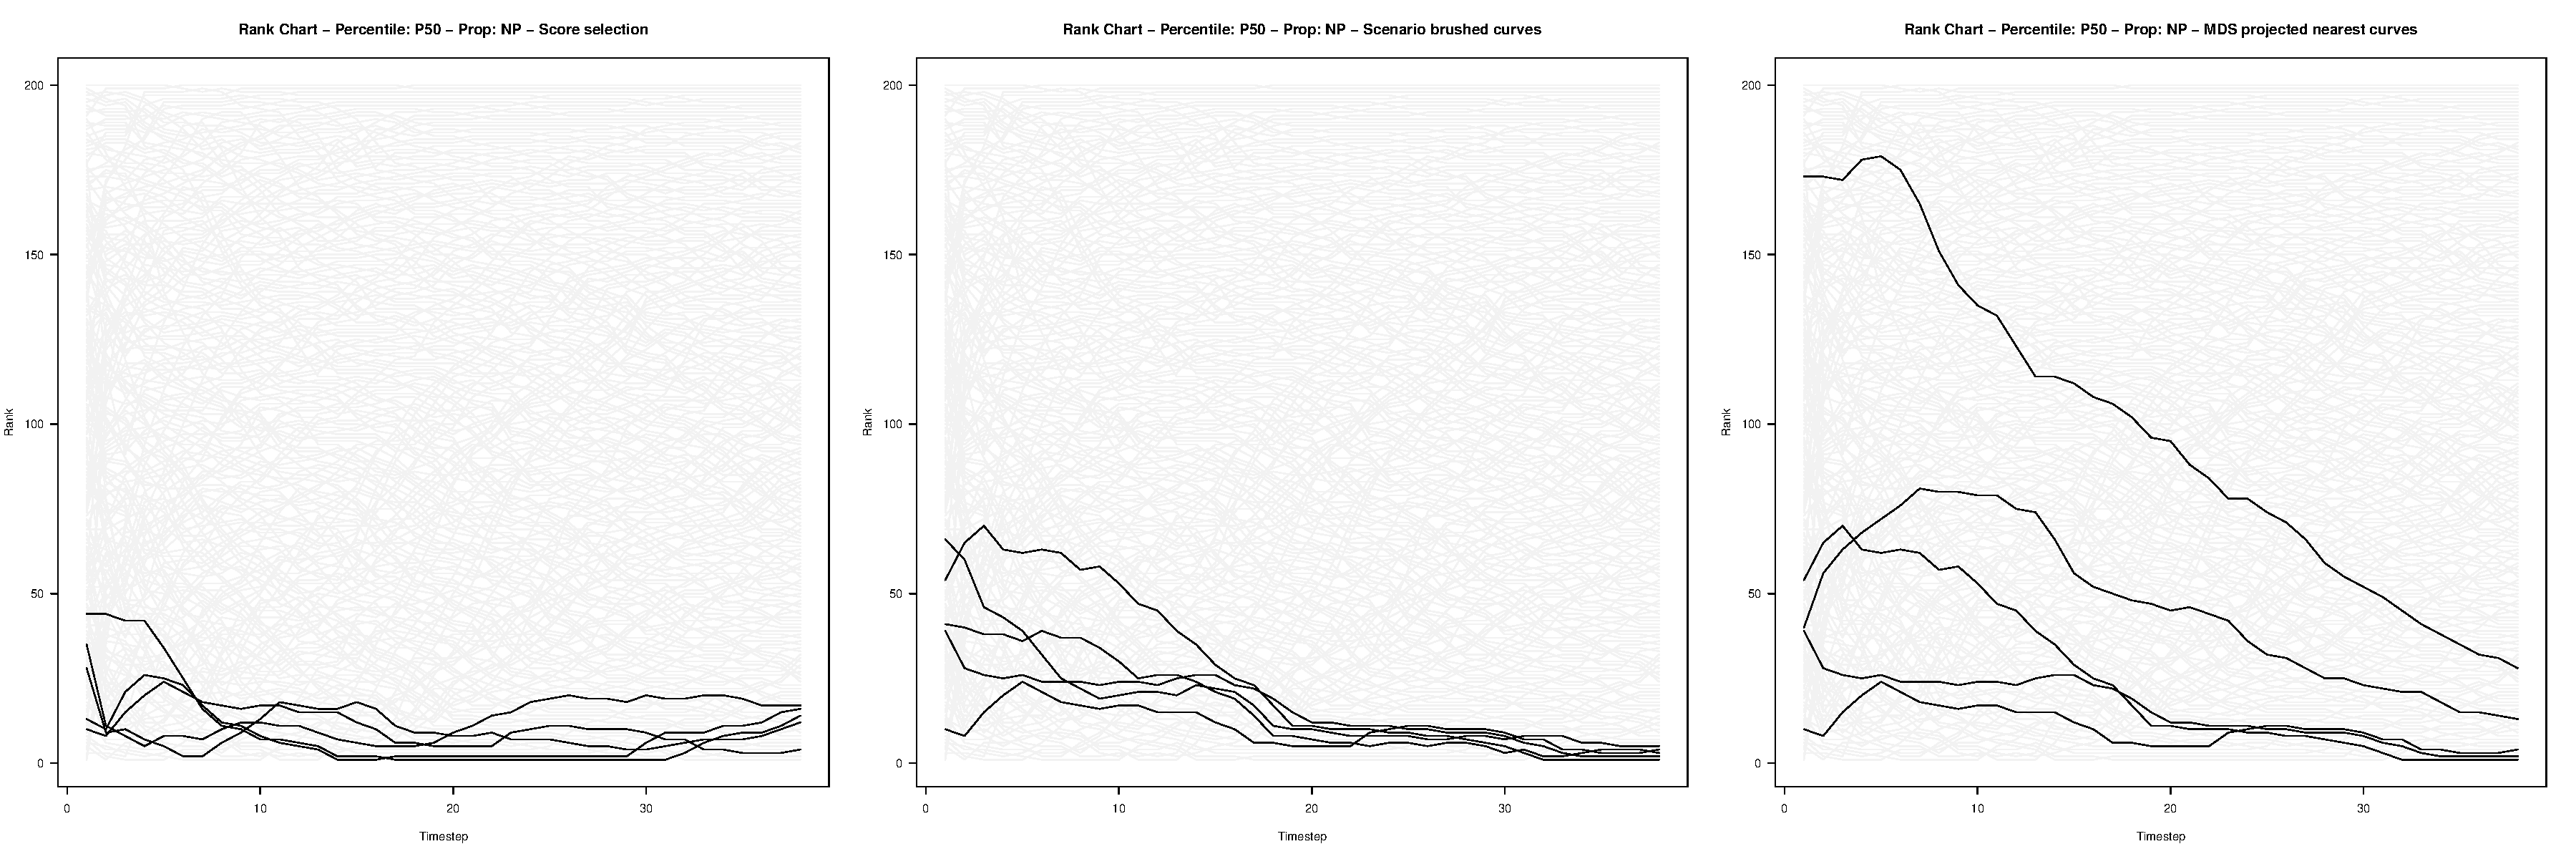
\includegraphics[width=\columnwidth]{rank-score-brush-mds-p50.pdf}
  \end{subfigure}
  \begin{subfigure}[b]{0.8\columnwidth}
    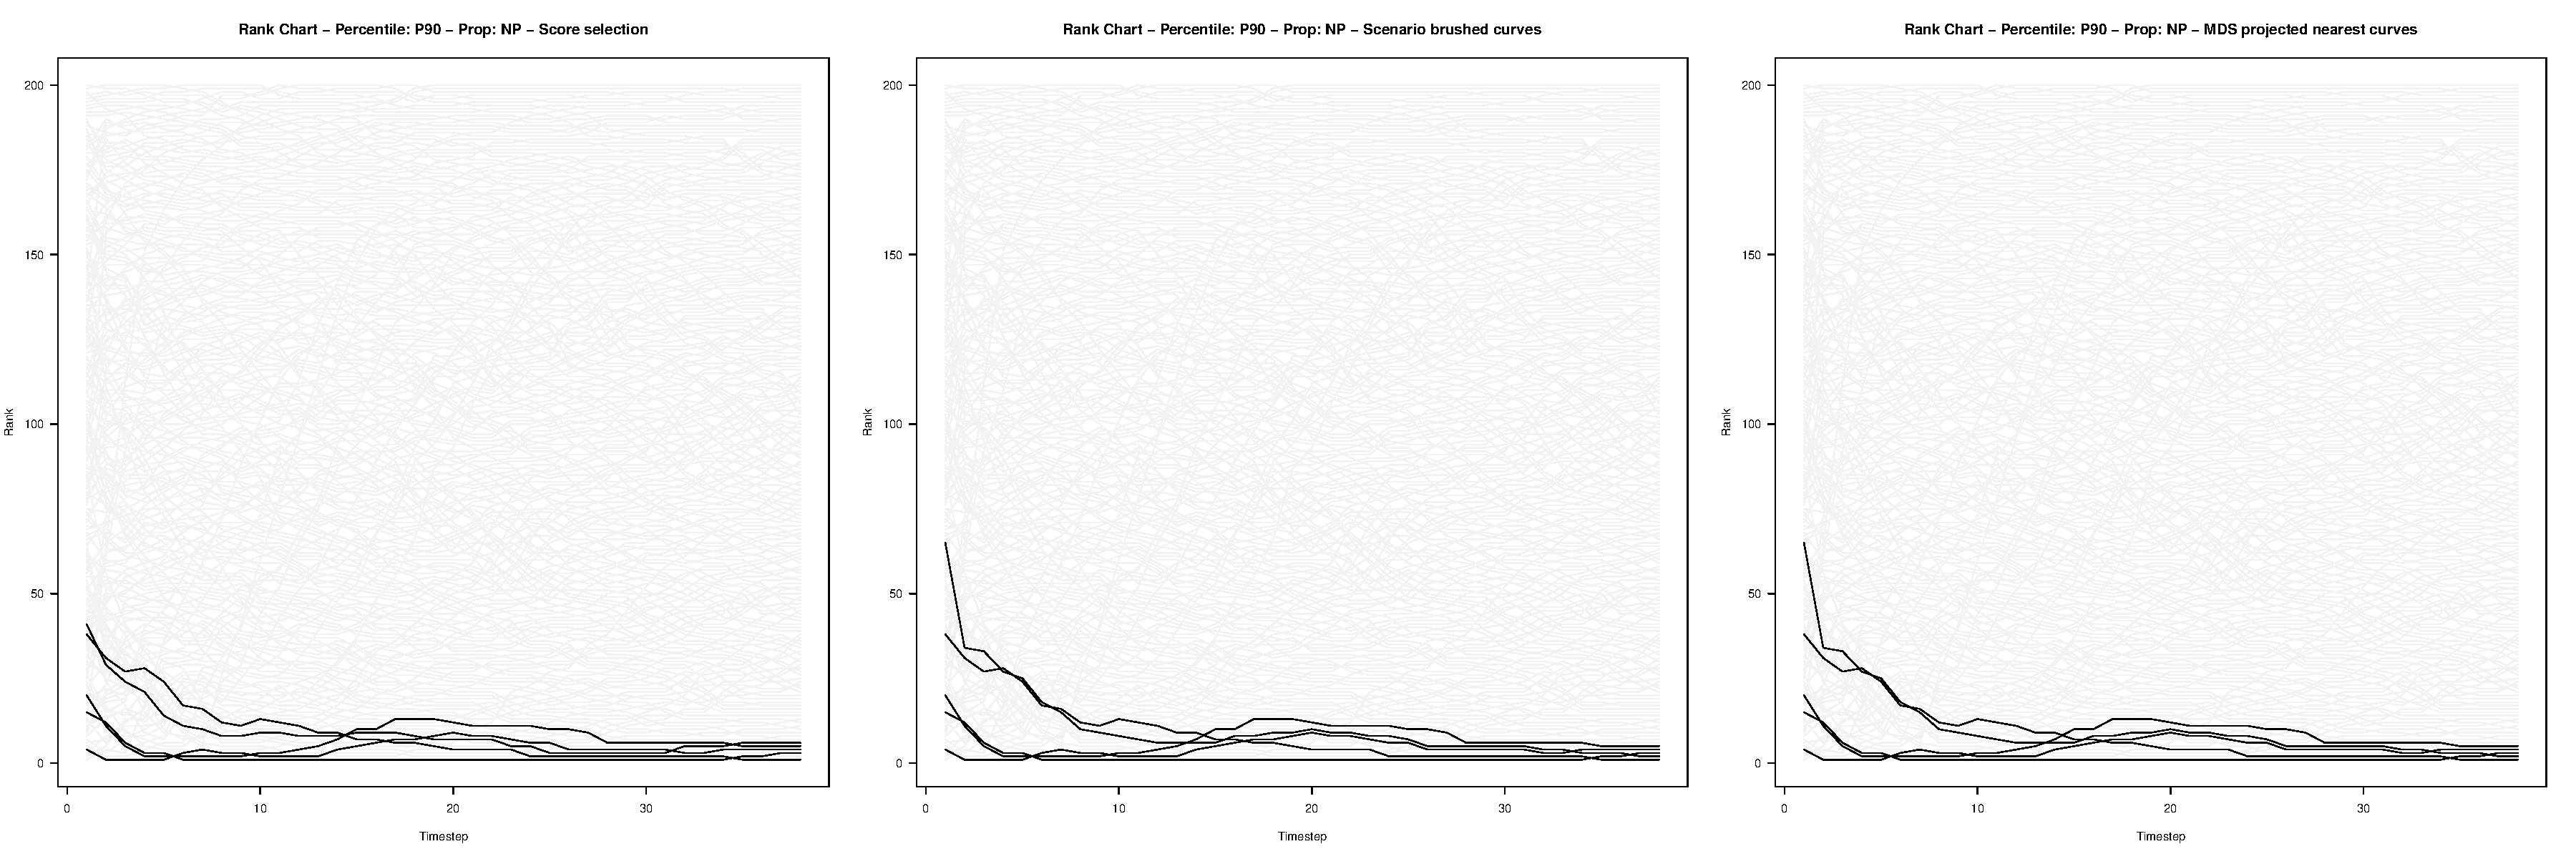
\includegraphics[width=\columnwidth]{rank-score-brush-mds-p90.pdf}
  \end{subfigure}
  \caption{Comparative rank charts of the selection methods employed.}
  \label{fig:rank-plots}
\end{figure}
\end{block}

%----------------------------------------------------------------------------------------

\end{column} % End of the first column

\begin{column}{\sepwid}\end{column} % Empty spacer column

\begin{column}{\twocolwid} % Begin a column which is two columns wide (column 2)

\begin{columns}[t,totalwidth=\twocolwid] % Split up the two columns wide column

\begin{column}{\twocolwid}\vspace{-.6in} % The second column within column 2 (column 2.2)

%----------------------------------------------------------------------------------------
%	RESULTS
%----------------------------------------------------------------------------------------

\begin{block}{Experimental Results}
\begin{figure}[H]
  \centering
  \begin{subfigure}[b]{0.8\columnwidth}
    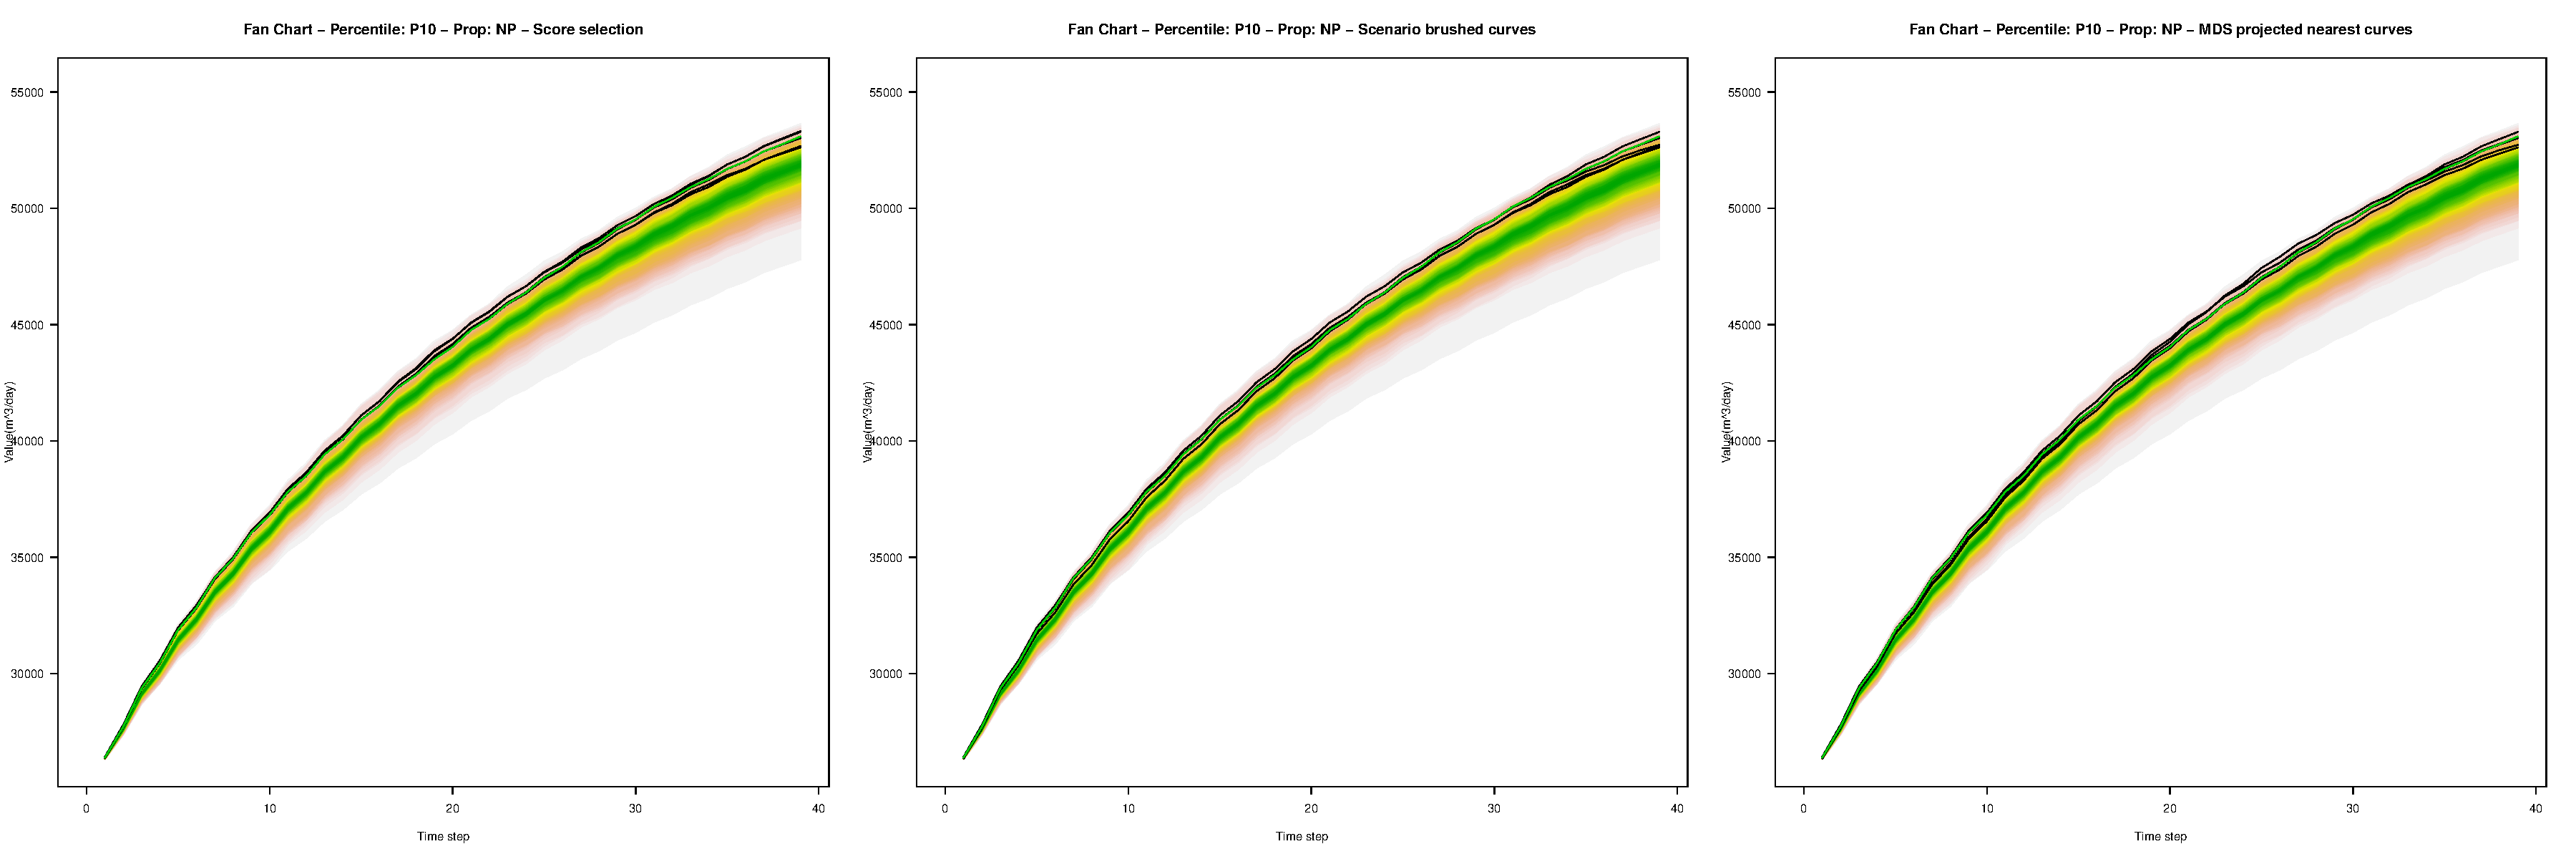
\includegraphics[width=\columnwidth]{fanchart-score-brush-mds-p10.pdf}
  \end{subfigure}
  \begin{subfigure}[b]{0.8\columnwidth}
    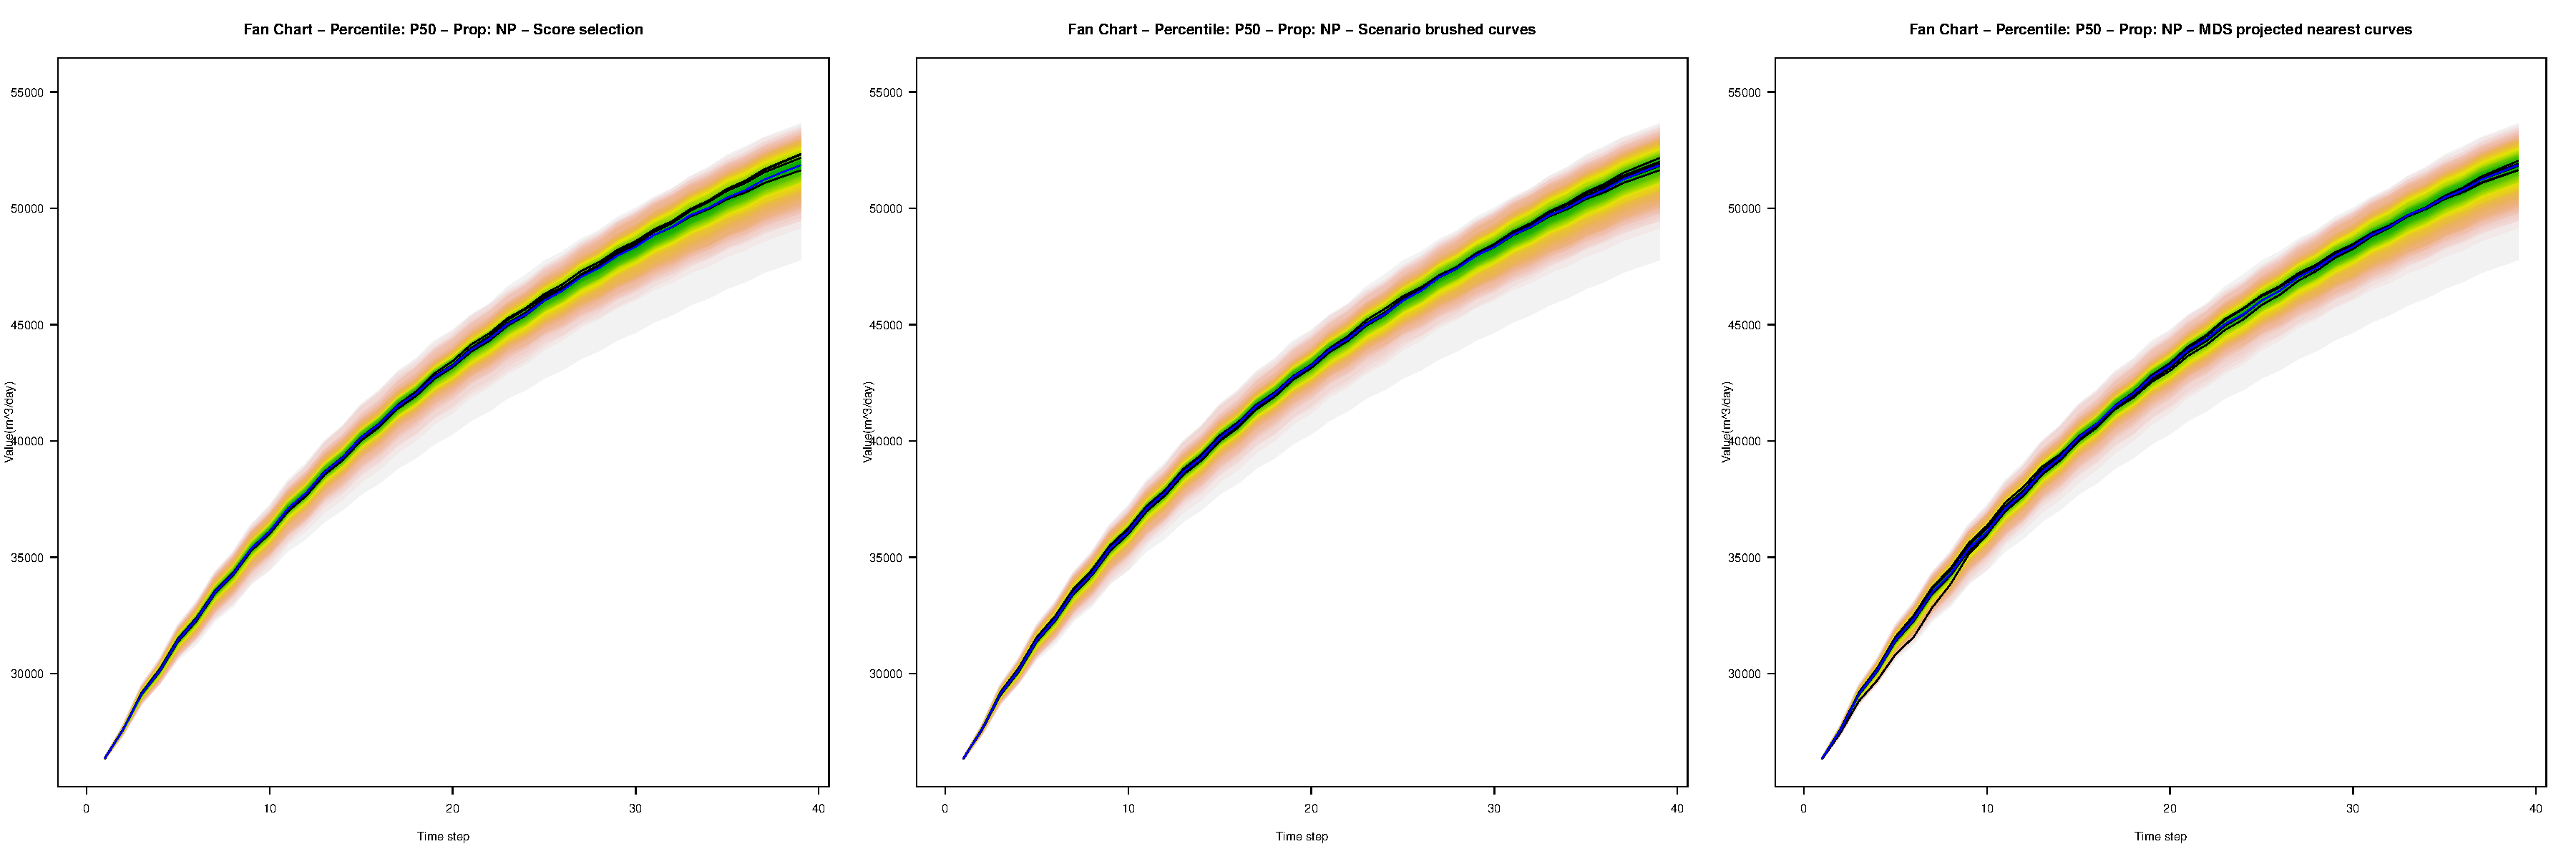
\includegraphics[width=\columnwidth]{fanchart-score-brush-mds-p50.pdf}
  \end{subfigure}
  \begin{subfigure}[b]{0.8\columnwidth}
    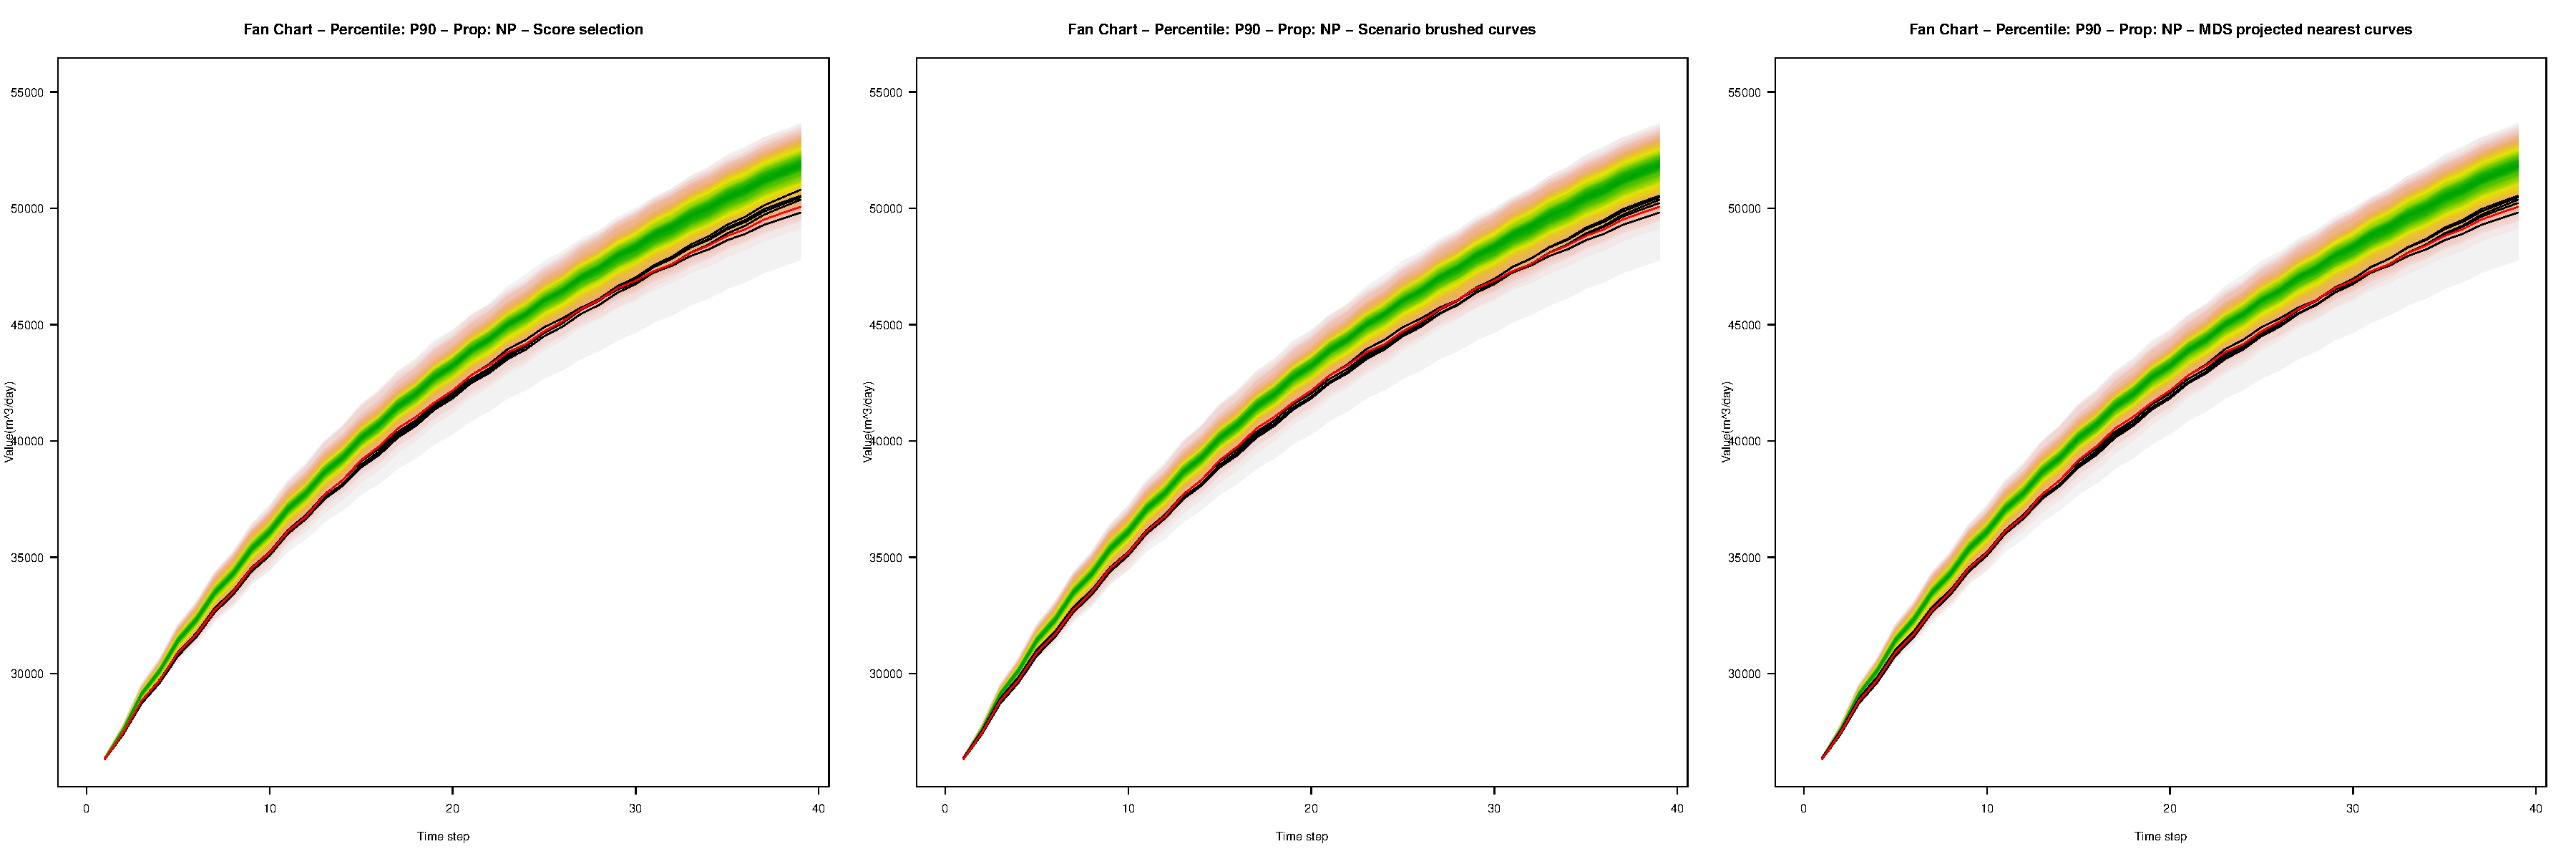
\includegraphics[width=\columnwidth]{fanchart-score-brush-mds-p90.pdf}
  \end{subfigure}
  \caption{Comparative fan charts of the selection methods employed.}
  \label{fig:fan-plots}
\end{figure}

The time series selected by the approaches employed have a good adherence to the percentile curve. With a notable exception of the MDS kNN selection in the P$_{50}$ case, every selected series has a good overall adherence to their references. The P$_{50}$ case seems to be the most problematic, as there are several series close to it. The score approach obtained the best set of candidades when compared to the manual and MDS results, with the MDS selection obtaining the worst overall series.
\end{block}

%----------------------------------------------------------------------------------------

%----------------------------------------------------------------------------------------
%	CONCLUSION
%----------------------------------------------------------------------------------------

\begin{block}{Conclusion}

In this work, we proposed an approach to select representative models for time series ensembles. To accomplish this task, we proposed a score function to automatically select a subset of time series as possible candidates. We tested our score function against a manual selection approach and a MDS $k$NN approach. The results indicate that our approach obtains a good set of possible candidates. We also developed a graphical tool, named rank chart, in order to evaluate the adherence of ensemble members to a reference curve.

When compared to previous works, our approach makes a significant contribution by dealing with a range of production values instead of handling only the final values. We found evidence that the past behavior of a model can impact on the selection process. We aim that our work sets an initial milestone to address this issue. However, our approach considers only one property when selecting the representative models. This may result in a sub-optimal selection when compared to other works \cite{selection-sarma:2013, meira:2016}.

\end{block}

\begin{block}{Future Work}
As a future work, we will validate our approach with expert users of such systems. We will look for ways to include multivariate time series in our analysis, in order to select representative candidates with respect to more properties at once. By including multivariate time series we must also look for ways to adapt the rank chart to represent them adequatly.
\end{block}


%----------------------------------------------------------------------------------------
%	REFERENCES
%----------------------------------------------------------------------------------------

\begin{block}{References}
%\nocite{*} % Insert publications even if they are not cited in the poster
\small{\bibliographystyle{unsrt}
\bibliography{references}\vspace{0.75in}}
\end{block}

%----------------------------------------------------------------------------------------
%	ACKNOWLEDGEMENTS
%----------------------------------------------------------------------------------------

\setbeamercolor{block title}{fg=red,bg=white} % Change the block title color

\begin{block}{Acknowledgements}
\small{\rmfamily{The authors would like to thank PETROBRAS for supporting this research. Guilherme Schardong, Waldemar Celes, Simone Barbosa and H\'elio Lopes would like also to thank CNPq for partially supporting their research.}} \\
\end{block}

%----------------------------------------------------------------------------------------

\end{column} % End of column 2.2

\end{columns} % End of the split of column 2

\end{column} % End of the second column

\end{columns} % End of all the columns in the poster

\end{frame} % End of the enclosing frame

\end{document}
